%%%%%%%%%%%%%%%%%%%%%%%%%%%%%%%%%%%%%%%%%%%%%%%%%%%%%%%%%%%%%%%%%%%%%%%%%%%%%%%%
%%  Rapport de Service, WorkflowManagement
%%%%%%%%%%%%%%%%%%%%%%%%%%%%%%%%%%%%%%%%%%%%%%%%%%%%%%%%%%%%%%%%%%%%%%%%%%%%%%%%
\documentclass[11pt, a4paper]{article}

\usepackage[english]{babel}
\usepackage[utf8]{inputenc}
\usepackage[T1]{fontenc}
\usepackage{amsfonts}
\usepackage{fancyhdr}
\usepackage[margin={2.5cm, 2.5cm}]{geometry}
\usepackage{graphicx}
\usepackage{pdfpages}
\usepackage{hyperref}
% \usepackage{algorithm2e}

\hypersetup{
  colorlinks,
  citecolor=black,
  filecolor=black,
  linkcolor=black,
  urlcolor=black
}

\newcommand\note[1]{\begin{quote}\emph{\textbf{Note : }}#1\end{quote}}

\pagestyle{empty}
\fancyhf{}
\renewcommand{\headrulewidth}{0pt}
\renewcommand{\footrulewidth}{0pt}
\lhead{Evaluating CRDTs for Real-time Document Editing}
\rhead{}
\lfoot{\today}
\cfoot{\thepage}
\rfoot{}

%%%%%%%%%%%%%%%%%%%%%%%%%%%%%%%%%%%%%%%%%%%%%%%%%%%%%%%%%%%%%%%%%%%%%%%%%%%%%%%%
%% Préambule
%%%%%%%%%%%%%%%%%%%%%%%%%%%%%%%%%%%%%%%%%%%%%%%%%%%%%%%%%%%%%%%%%%%%%%%%%%%%%%%%
\title{ Summary
       <<Evaluating CRDTs for Real-time Document Editing>>}

\author{Ronan-Alexandre Cherrueau\\Adrien Bougouin\\Alban Ménager}
\date{Year 2011-2012\\
      (University of Nantes)}
\makeindex

%%%%%%%%%%%%%%%%%%%%%%%%%%%%%%%%%%%%%%%%%%%%%%%%%%%%%%%%%%%%%%%%%%%%%%%%%%%%%%%%
%% Début
%%%%%%%%%%%%%%%%%%%%%%%%%%%%%%%%%%%%%%%%%%%%%%%%%%%%%%%%%%%%%%%%%%%%%%%%%%%%%%%%
\begin{document}
  \maketitle

  \fancypagestyle{plain}{\fancyhead{} \fancyfoot{}} 
  %\vfill
  %\tableofcontents\renewcommand{\headrulewidth}{0.4pt}
  ~\newline
  \renewcommand{\footrulewidth}{0.4pt}
  \pagestyle{fancy}
  \fancypagestyle{plain}{}
  \newpage

  %%%%%%%%%%%%%%%%%%%%%%%%%%%%%%%%%%%%%%%%%%%%%%%%%%%%%%%%%%%%%%%%%%%%%%%%%%%%%%
  Nowadays, colaboring work is increasing and real-time editing systems are catching on. Google Docs is a good example, since it enables multiple authors to edit the same document at the same time, whenever it is and wherever they are.
  
  %%%%%%%%%%%%%%%%%%%%%%%%%%%%%%%%%%%%%%%%%%%%%%%%%%%%%%%%%%%%%%%%%%%%%%%%%%%%%%
  For now, real-time editing systems use a replication mechanism to ensure consistency when merging concurrent changes performed on the same document. Optimistic replication gives to users a low time of latency. But they use centralise approaches and the probleme with this is that it's not only storing documents information but personal informations too and it could be a privacy threat if they are used by corporations.
  
  %%%%%%%%%%%%%%%%%%%%%%%%%%%%%%%%%%%%%%%%%%%%%%%%%%%%%%%%%%%%%%%%%%%%%%%%%%%%%%
  So, to prevent this, a good solution for not using centralized mechanisms is to replace them by an decentralized ones. So, peer-to-peer seems to be a solution. Nevertheless, the main key factor is performance. Obviously, if the editing applications can't respond to users' actions in a reasonable time (about 50ms), they may get frustrated and stop the current application.

  %%%%%%%%%%%%%%%%%%%%%%%%%%%%%%%%%%%%%%%%%%%%%%%%%%%%%%%%%%%%%%%%%%%%%%%%%%%%%%
   The goal of this experiments is to select some algorithms based on optimistic replication and evaluate them on a decentralized real-time collaborative editing system. The evaluations will be based on real context on the sames conditions and using the same data flow.

The first approach is \emph{Operation Transformation}. This approche takes into account the effect of concurrents operations. An \emph{Operation Transformation} is used to keep document consistency after severals concurrents operations. Google Docs use an algorithm named \emph{Jupiter} and use a vector clock to detect concurrents operations, but this solution doesn’t get on well in the peer-to-peer system.

A new approach called \emph{Commutative Replicated Data Types} (CRDT) for peer-to-peer environment was introduced as a new class of replication mechanisms to preserve consistency. CRDT doesn't required concurrent operations detections because it's designed for concurrent operations to be natively commutative.

  %%%%%%%%%%%%%%%%%%%%%%%%%%%%%%%%%%%%%%%%%%%%%%%%%%%%%%%%%%%%%%%%%%%%%%%%%%%%%%
  CRDT have some caracteristic:
\begin{itemize}
	\item The concurrent operations are natively commutative.
	\item The document is a linear sequence of elements.
	\item A unic position identifier.
\end{itemize}~

For the experiments, they select differents algorithms for generating the unic position identifier:
\begin{itemize}
	\item Logoot
	\item RGA
	\item WOOT
	\item WOOTO
	\item WOOTH
\end{itemize}

Figure \ref{fig:worst} p.\pageref{fig:worst} (with R the number of replicas and by H the number of operations on the document) shows the theoretical evaluation of this differents algorithms. RGA and Logoot have the bests results.

\begin{figure}[h]
  \center
  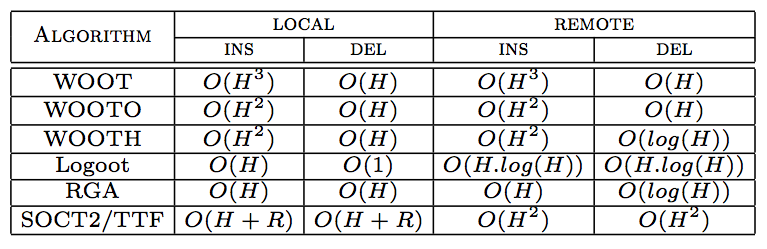
\includegraphics[width=0.7\textwidth]{includes/worst.png}
  \caption{Worst-case time-complexity analysis}
  \label{fig:worst}
\end{figure}
  
  %%%%%%%%%%%%%%%%%%%%%%%%%%%%%%%%%%%%%%%%%%%%%%%%%%%%%%%%%%%%%%%%%%%%%%%%%%%%%%
  But this is just theoretical. The team who wrote the paper designed real-time peer-to-peer collaborations application in order to obtain their logs and apply them on the algorithms. About the real applications, two experiments and several groups have been made:
\begin{itemize}
	\item 3 groups have to do their semester report by only using the collaborating editor for one hour and a half:
		\begin{itemize}
			\item 2 groups of 4 students.
			\item 1 group of 5 students.
		\end{itemize}
	\item 9 groups of 2 students have to translate an episode of \emph{The Big Bang Theory}
\end{itemize}~

Figure \ref{fig:operations} p.\pageref{fig:operations} shows the amount of users/character operations:
\begin{itemize}
	\item A user operation is adding/deleting letters or groups (copy/past).
	\item A character operation is the transformation of each user operation into a character operation (for example, copy/past "alma" are the character operations: \begin{itemize}
					\item adding 'a' at space 0
					\item adding 'l' at space 1
					\item ...
				\end{itemize}
\end{itemize}~

\begin{figure}[h]
  \center
  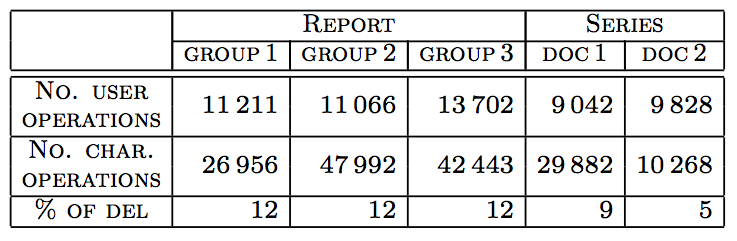
\includegraphics[width=0.7\textwidth]{includes/operations.png}
  \caption{Total number of user/character operations}
  \label{fig:operations}
\end{figure}
  
  %%%%%%%%%%%%%%%%%%%%%%%%%%%%%%%%%%%%%%%%%%%%%%%%%%%%%%%%%%%%%%%%%%%%%%%%%%%%%%
  All the algorithms have been runned 10 times with same data and the same conditions. Figures \ref{fig:users_operations_2g_report} and \ref{fig:users_operations_1t_big} p.\pageref{fig:users_operations_2g_report} shows the total number of users operations.

%\begin{figure}
%	\center
%  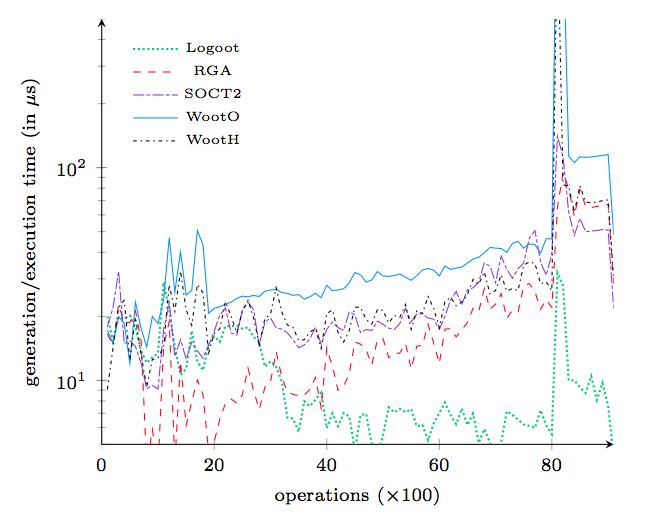
\includegraphics[width=0.6\textwidth]{includes/users_operations_1t_big.png}
%  \caption{User operation execution times - 1st series}
%  \label{fig:users_operations_1t_big}
%\end{figure}  
%\begin{figure}
%	\center
%  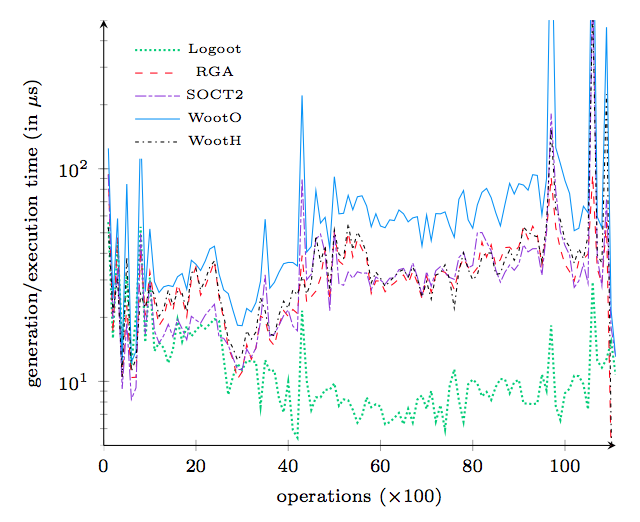
\includegraphics[width=0.6\textwidth]{includes/users_operations_2g_report.png}
%  \caption{User operation execution times - 2nd group
%report}
%  \label{fig:users_operations_2g_report}
%\end{figure}

\begin{figure}[h]

\begin{minipage}{0.50\linewidth}
  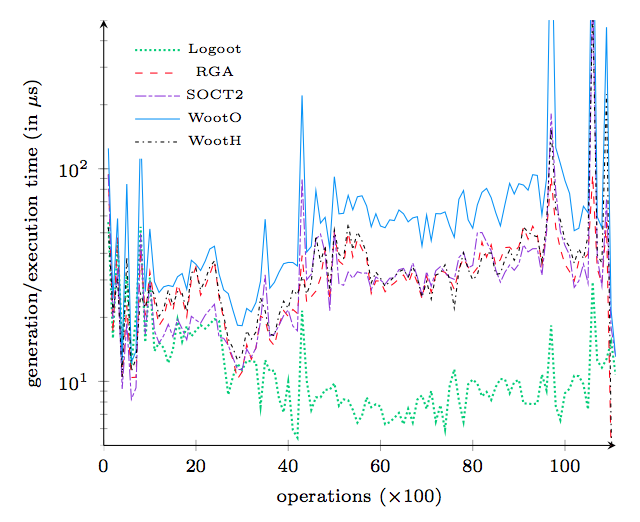
\includegraphics[width=1.2\textwidth]{includes/users_operations_2g_report.png}
  \caption{User operation execution times - 2nd group
report}
  \label{fig:users_operations_2g_report}
  \end{minipage} \hfill
  \begin{minipage}{.50\linewidth}
    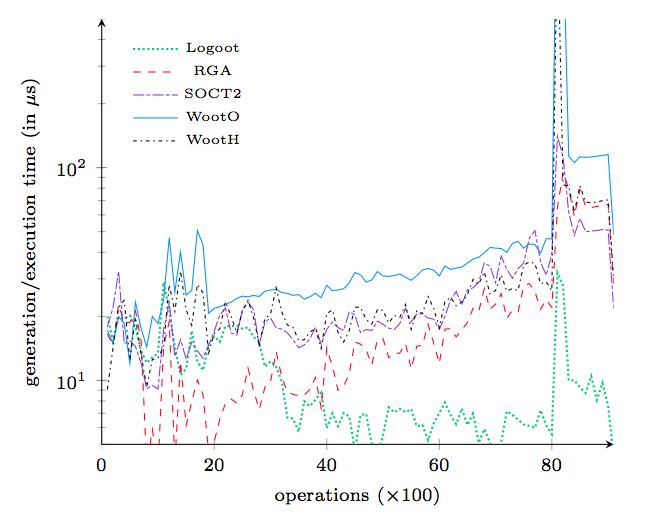
\includegraphics[width=1.2\textwidth]{includes/users_operations_1t_big.png}
  	\caption{User operation execution times - 1st series}
  	\label{fig:users_operations_1t_big}
\end{minipage} \hfill
\end{figure}

The increases are due to insert or delete a large group of characters on the document. All the algorithms decrease over the time because of the size of the document (the unique identifier gets bigger when there are a lot of operations) but logoot decreases slowly compared to the others.\\

Figures \ref{fig:characters_operations_2g_report} and \ref{fig:characters_operations_1t_big} p.\pageref{fig:characters_operations_2g_report} shows the total number of characters operations.

\begin{figure}[h]
\begin{minipage}{0.50\linewidth}
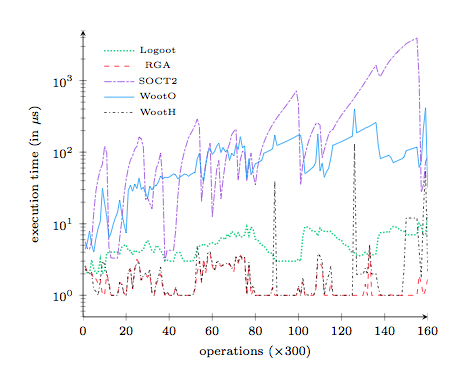
\includegraphics[width=1.2\textwidth]{includes/characters_operations_2g_report.png}
  \caption{Character operation execution times - 2nd
group report}
  \label{fig:characters_operations_2g_report}
  \end{minipage} \hfill
  \begin{minipage}{.50\linewidth}
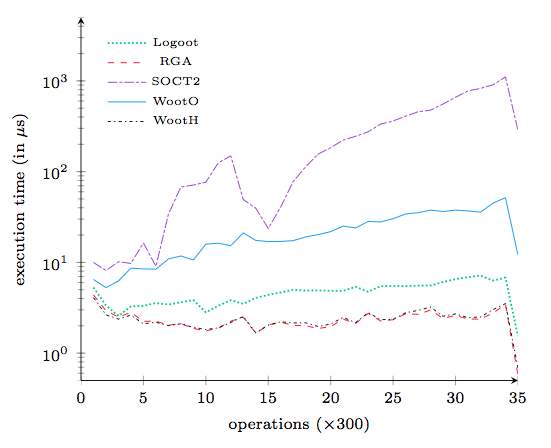
\includegraphics[width=1.2\textwidth]{includes/characters_operations_1t_big.png}
  \caption{Character operation execution times - 1 time
series}
  \label{fig:characters_operations_1t_big}
\end{minipage} \hfill
\end{figure}

Wooto, Logoot and RGA remains stable during al the time. The behavior of SOCT2 performance is mainly due to its garbage collection mechanism. Users have a period of inactivity and the garbage mechanism cannot purge the history log. SOCT2 can't be used for real-time editing because of his response time increasing 50ms quickly.\\

Figure \ref{fig:characters_operations_2g_report} is a bite different than \ref{fig:characters_operations_1t_big} because of the number of characters deletes (students didn't delete as much as in the serie experiments as in the report experiment). RGA and WootH are better than the others because their algorithms are based on hash tables.\\


  
  %%%%%%%%%%%%%%%%%%%%%%%%%%%%%%%%%%%%%%%%%%%%%%%%%%%%%%%%%%%%%%%%%%%%%%%%%%%%%
  \chapter*{Conclusion}
\addcontentsline{toc}{chapter}{Conclusion}
  \begin{itemize}
    \item Rappel du sujet.
    \item Bilan du travail effectué.
    \item
    \item
  \end{itemize}


\end{document}

